\subsection{Solutions and Colligative Properties}
\textbf{Solution}: Homogeneous mixture of two ro more substances \hspace{3pt}
\fbox{solution $=$ solvent $+$ solute(s)}\\

\textbf{Precipitation Reaction}: Reactions that result in the formation of an insoluable product are called precipitation reactions.\\
\textbf{e.g.} $Ag(NO_3)(aq) + KCl(aq) \longrightarrow AgCl(s) + KNO_3 (aq)$ \hspace{3pt} $AgCl$ is the solid precipitate\\

\textbf{Ionic Equations}\\
\textbf{1. Comple Ionic eq.} \textbf{e.g.}$Ag^{+}(aq) + NO_3^{-}(aq) + K^{+}(aq) + Cl^{-}(aq) \longrightarrow AgCl(s) + K^{+}(aq) + NO_3^{-}$\\
$K^{+}(aq)$ and $NO_3^{-}(aq)$ are spectator ions\\
\textbf{2. Net Ionic eq.} \textbf{e.g.} $Ag^{+}(aq) + Cl^{-}(aq) \longrightarrow AgCl(s)$

\begin{minipage}{0.6\linewidth}
    \begin{center}
        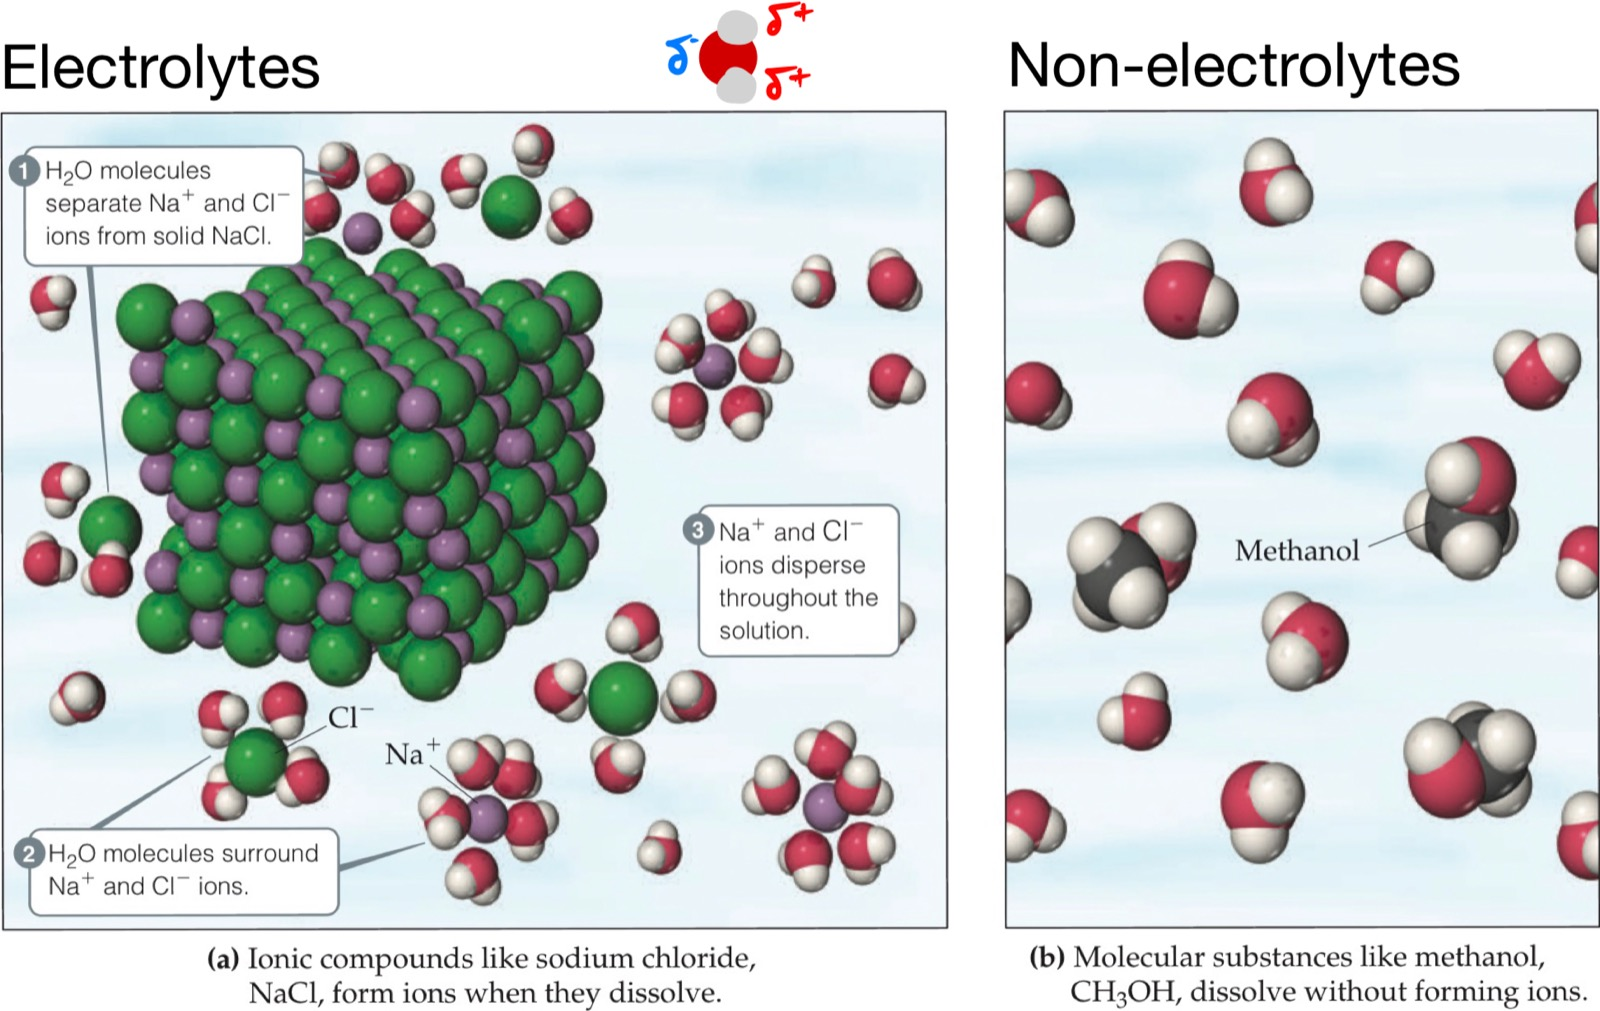
\includegraphics[width = 0.9\linewidth]{images/electrolytes_non_electrolytes.jpeg}
    \end{center}
\end{minipage}
\begin{minipage}{0.39\linewidth}
    \begin{center}
    \textbf{Neutralization Reaction}
        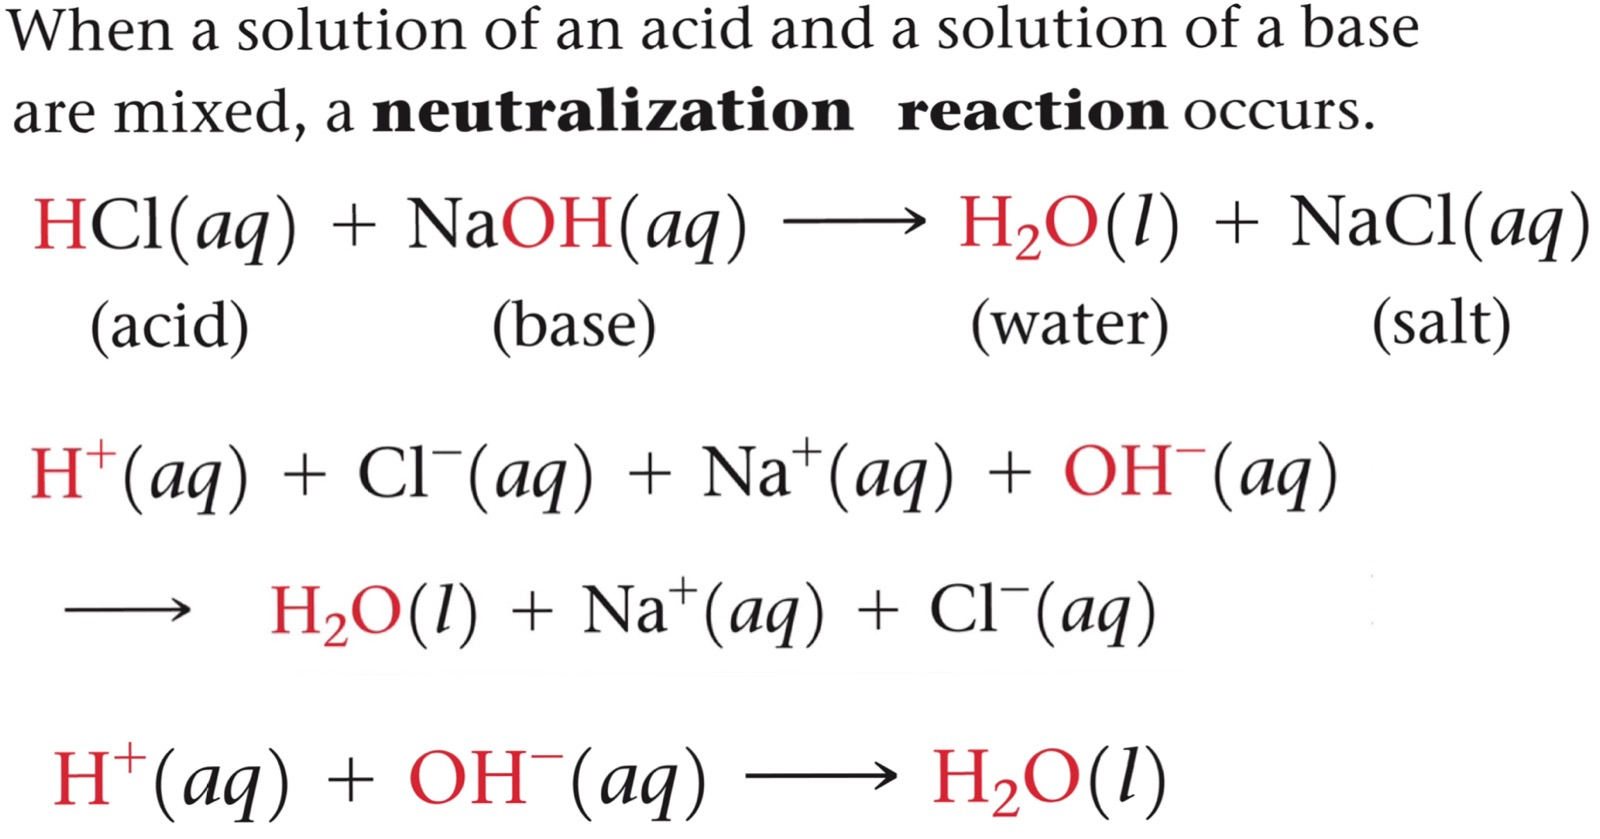
\includegraphics[width = \linewidth]{images/neutralization_reaction.jpeg}
    \end{center}
    \textbf{Concentration}\\
    \fbox{Molarity $= \frac{\text{moles solute}}{\text{volume of solution in L}}$}
\end{minipage}
\textbf{Thermodynamics of Solutions}\\
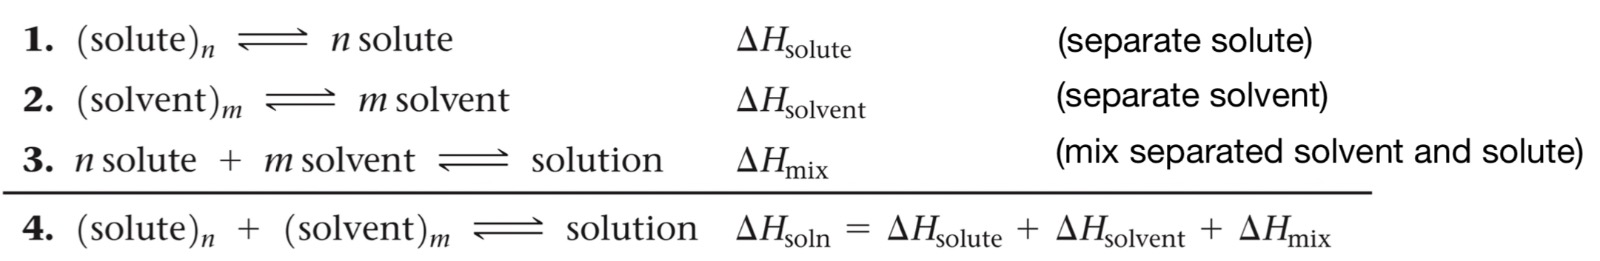
\includegraphics[width = 0.8\linewidth]{images/solvent_solution.jpeg}
\begin{center}
   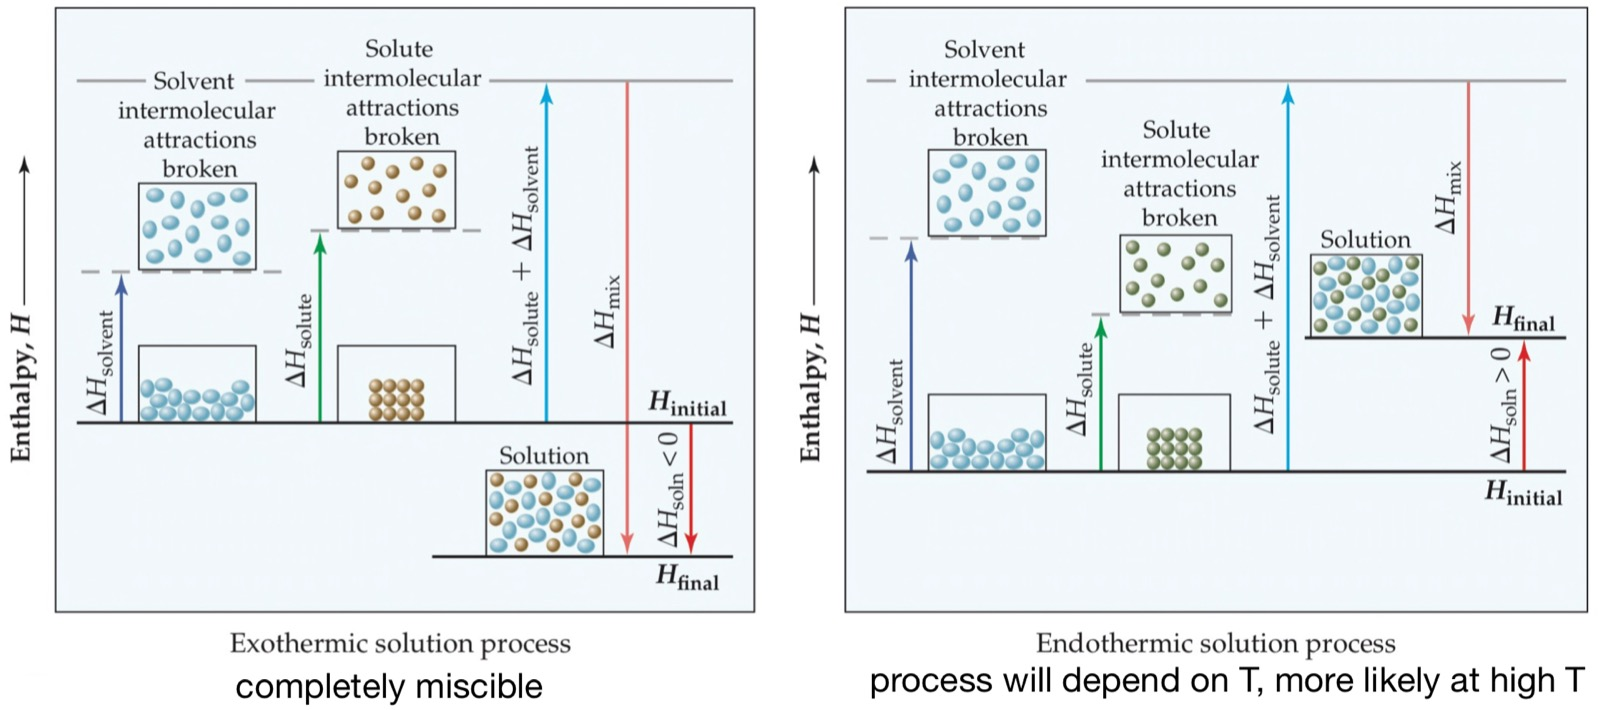
\includegraphics[width = 0.9\linewidth]{images/miscible_not_miscible.jpeg} 
   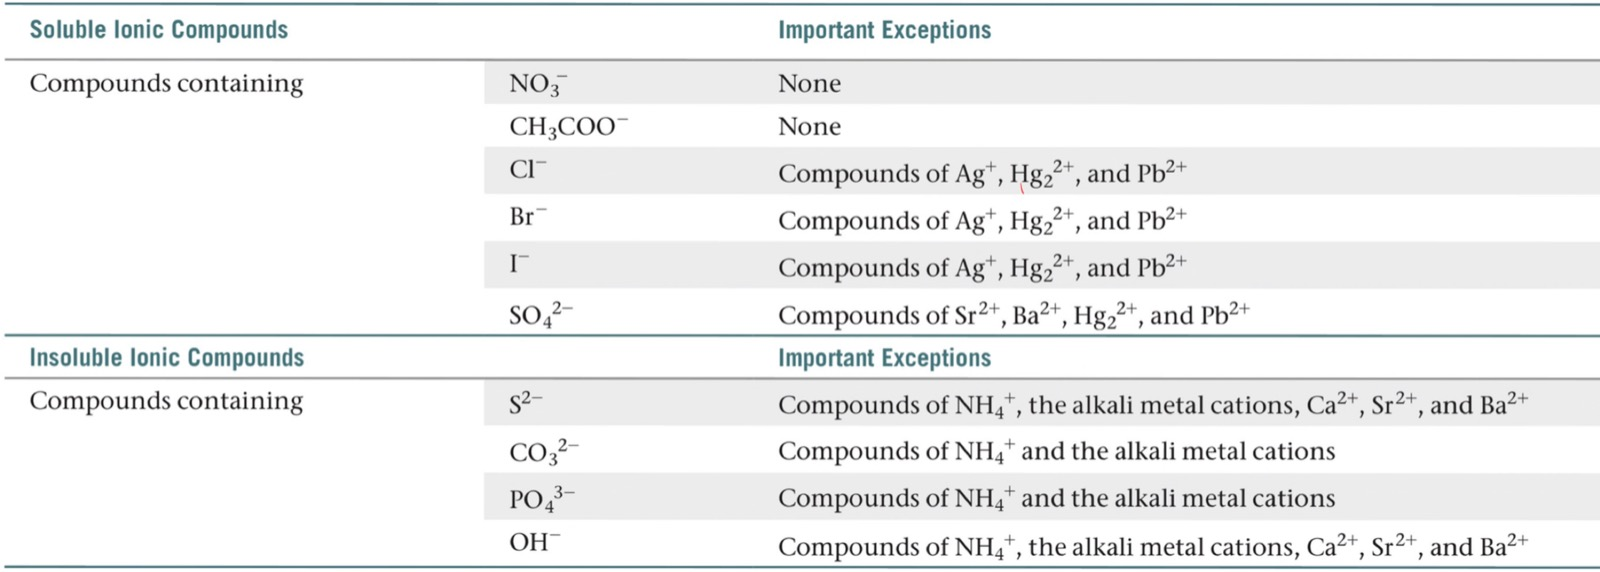
\includegraphics[width = 0.95\linewidth]{images/soluibility.jpeg}
\end{center}
\begin{minipage}{0.2\linewidth}
    \textbf{Gas Solubility}\\
    \fbox{$S_g = kP_g$}
\end{minipage}
\begin{minipage}{0.79\linewidth}
    \textbf{k}: Henry's law constant $[k] = \frac{mol}{m^3\cdot Pa}$, dependent on solute and solvent\\
    \textbf{$P_g$}: Gas partial pressure above liquid $[P_g] = Pa$
\end{minipage}
\textbf{Colligative Properties}\\
Changes only depend on the amount of solute added and not the type of solute\\
\begin{minipage}{0.35\linewidth}
    \textbf{1. Boiling-Point Elevation}\\
    \fbox{$\Delta T_b = T_b$(solution)$- T_b$(solvent) $= i K_b m$}\\
    $m \equiv$ molalilty of solute\\
    $k_b \equiv$ molal bp. elevation constant\\
    $i \equiv$ van't Hoff factor ($NaCl \longrightarrow i = 2$)
\end{minipage}
\begin{minipage}{0.32\linewidth}
    \textbf{2. Vapor-Pressure Lowering \\(Raoult's Law)}\\
    \fbox{$P_{vap}^{sol} = X_{solvent} \cdot P_{vap}^{pure}$}\\
    $P_{vap}^{sol} \equiv$ vapour pressure of solution\\
    $X_{solvent} \equiv$ mole fraction solvent\\
    $P_{vap}^{pure} \equiv$ vapour pressure of pure solvent 
\end{minipage}
\begin{minipage}{0.32\linewidth}
    \textbf{3. Freezing-Point Depression}\\
    \fbox{$\Delta T_f = T_f$(solution)$- T_f$(solvent) $= -i K_f m$}\\
    $m \equiv$ molalilty of solute\\
    $k_f \equiv$ molal fp. depression constant\\
    $i \equiv$ van't Hoff factor
\end{minipage}

